\scanpage{210}
Le système de groupes \inserted{sur $\mathbb{Q}$} (36, 37), muni
de l'hom de
\[
\Pi \subset \mathcal{G} \subset M
\]
dans \deleted{\unsure{$\mathcal{G}$}}
\[
(40)\qquad
\underline{\Pi}_{\mathbb{Q}}(\unsure{\mathbb{A}'_{\mathbb{Q}}})
\subset \underline{\mathcal{G}}_{\mathbb{Q}}(\mathbb{A}_{\mathbb{Q}})
\subset \underline{M}_{\mathbb{Q}}(\unsure{\mathbb{A}_{\mathbb{Q}}})
\]
\deleted{déduit} \inserted{induit} par
$M\longrightarrow \unsure{G}(\mathbb{A}_{\mathbb{Q}})$ (satisfaisant
aux conditions $1^\circ)$ à $4^\circ)$ ci-dessus \deleted{\unsure{)}}, i.e.
d'un ``hom de Lie'') s'appellera aussi
une ``\uline{approximation de Lie}'' du
système de Galois-Teichmüller envisagé.

Considérons un \deleted{germe d'}hom
\[
(41)\qquad k_i^{\deleted{\unsure{\sharp}}}\quad T_0\longrightarrow\Pi_0
\]
\unsure{appartenant|correspondant} à la L-structure de $\Pi$,
définit donc \inserted{par composition avec
$\unsure{\Pi_0}\longrightarrow
\deleted{\unsure{\mathcal{G}}}\underline{\Pi}_{\deleted{\unsure{\mathbb{Q}}}}(\mathbb{Q})$}
un \deleted{germe d'}homomorphisme
\[
(42)\qquad T_0\longrightarrow
\deleted{\unsure{\mathcal{G}}}\underline{\Pi}(\mathbb{Q}).
\]
\margin{\uline{NB} pour $i$ fixé,
$k_i$ est déterminé mod
\unsure{autom.} int. de $\Pi_0$ \uuline{et}
mod composition avec
$n\,\mathrm{id}_{T_0}$, pour $n\in\mathbb{N}^{*}$.
Pour ce qui est de ce dernier point, \unsure{il y a}
\unsure{souvent} (\unsure{fixons} $\Pi_0$) un
``meilleur choix'', dont tous \unsure{les autres se}
déduisent par composition avec
$n\,\mathrm{id}_{T_0}$.}
On voit \inserted{((21) p.\,$747'$)} que cet \deleted{germe de} homomorphisme
est quasi-unipotent, et qu'il définit par
suite un hom de \deleted{\unsure{g}} schémas en groupes
\margin{209}

\scanpage{211}
\mspage{753}
\[
(43)\qquad \underline{k}_i:
\underset{(\simeq G_{a\mathbb{Q}}\otimes_{\mathbb{Z}}T_0)}{\underline{T}_{0\mathbb{Q}}}
\longrightarrow \underline{\Pi}_{\mathbb{Q}}
\]
(pas seulement un germe!)
qui définit, par \deleted{composition} passage aux
pts $\mathbb{Q}$-rationnels, le \uline{germe} d'hom
(42). On trouve ainsi un ens. fini
(indexé par \inserted{l'ens} des germes de \uline{sous-groupes}
lacets de $\Pi_0$, ou de $\Pi$ ce qui revient \unsure{au}
$\unsure{\overline{\mathrm m}}$) des hom extérieurs (43) de schémas
en groupes. J'ai envie d'appeler l'appro-\deleted{\unsure{représentation}}\inserted{ximation} de Lie \uline{non dégénérée} si
les hom précédents sont tous non
triviaux, donc sont des \uline{mono.}
\[
(44)\qquad \underline{k}_i:
\underline{T}_{0\mathbb{Q}}\simeq G_{a\mathbb{Q}}\otimes_{\mathbb{Z}}T_0
\lhook\joinrel\longrightarrow \underline{\Pi}_{\mathbb{Q}}.
\]

Supposons que $\underline{M}_{\mathbb{Q}}$ provienne
d'un schéma en groupes (affine \unsure{et} t.f.)
$\underline{M}$ sur $\mathbb{Z}$, tel que l'on ait
\[
(45)\qquad M\longrightarrow\underline{M}(\widehat{\mathbb{Z}})
\]
(il me semble qu'on peut tjrs trouver un
tel $\underline{M}$...). On désigne alors par
\margin{210}

\scanpage{212}
$\underline{\Pi}$, $\underline{\mathcal{G}}$ les adhérences schématiques dans
$\underline{M}$ de $\underline{\Pi}_{\mathbb{Q}}$, $\underline{\mathcal{G}}_{\mathbb{Q}}$, d'où un diagramme
de schémas en groupes sur $\mathbb{Z}$
\[
(46)\qquad
\diagram{\begin{tikzcd}[ampersand replacement=\&,column sep=3em]
\underline{\Pi}
\arrow[r,phantom,"\subset" description]
\arrow[r,no head,to path={(\tikztostart.north) -- ++(0,0.35) -| (\tikztotarget.north) \tikztonodes},"\underline{\unsure{\mathcal{T}}}"]
\arrow[rr,no head,to path={(\tikztostart.south) -- ++(0,-0.35) -| (\tikztotarget.south) \tikztonodes},"\underline{N}"']
\&\underline{\mathcal{G}}
\arrow[r,phantom,"\subset" description]
\arrow[r,no head,to path={(\tikztostart.north) -- ++(0,0.35) -| (\tikztotarget.north) \tikztonodes},"\underline{\Gamma}"]
\&\underline{M}
\end{tikzcd}}
\]
(sous réserve de représentabilité des
quotients $\underline{\unsure{\mathcal{T}}}$, $\underline{\Gamma}$, $\underline{N}$ --- mais je crois que
pour Raynaud il n'y a jamais de pb...).
On \deleted{\unsure{va supposer|suppose} bien sûr que}
\inserted{aura des factorisations}
\[
(47)\qquad
\diagram{\begin{tikzcd}[ampersand replacement=\&,column sep=large,row sep=large]
\Pi_0\arrow[r,hook,no head]\arrow[d]
\&\mathcal{G}_0\arrow[r,hook]\arrow[d]
\&M\arrow[d]\\
\underline{\Pi}(\mathbb{Z})\arrow[r,hook]
\&\underline{\mathcal{G}}(\mathbb{Z})\arrow[r,hook,no head]
\&\underline{M}(\widehat{\mathbb{Z}}).
\end{tikzcd}}
\]

On suppose bien sûr \deleted{\unsure{(y a-t-il}} que
l'hom $\chi_{\underline{\unsure{M}}}:\deleted{\unsure{\mathbb{Q}}}\underline{M}_{\mathbb{Q}}\longrightarrow G_{m\mathbb{Q}}$ se
prolonge en
\[
(48)\qquad \chi_{\underline{M}}:\underline{M}\longrightarrow G_{m\mathbb{Z}},
\]
lequel évidemment se factorise par
\[
(49)\qquad \chi_{\underline{\Gamma}}:\underline{\Gamma}\longrightarrow G_{m\mathbb{Z}}.
\]
\margin{211}


\scanpage{213}
\mspage{754}
Il serait intéressant de dégager un th. d'existence,
(voir \inserted{\unsure{même}} d'unicité, moyennant des conditions plus fortes
encore) d'un ``modèle'' $\underline{M}$ \inserted{\uline{lisse}} sur $\mathbb{Z}$ de $\underline{M}_{\mathbb{Q}}$,
satisfaisant aux conditions précédentes
\figure{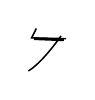
\begin{tikzpicture}[x=0.5cm,y=0.5cm,baseline=0]
\draw[line width=0.55pt] (0.12,0.72)--(0,0.48)--(0.88,0.46);
\draw[line width=1pt] (0.06,0.46)--(0.82,0.43);
\draw[line width=0.55pt] (0.75,0.53) .. controls (0.48,0.16) and (0.18,-0.2) .. (-0.08,-0.36);
\end{tikzpicture}}
\[
(M\longrightarrow\underline{M}(\mathbb{Z}),\quad
\text{et }\underline{M}\xrightarrow{\chi_{\underline{M}}}G_{m\mathbb{Z}}).
\]

Ici il ne sera plus vrai en général, je
présume, que les hom. extérieurs \inserted{$\underline{k}_i$} (43) se
prolongent tels quels en des hom
$\underline{T}_i\underset{\unsure{\mathrm{df}}}{=}\underline{T}_{i\mathbb{Z}}\longrightarrow\underline{\Pi}$.
Mais je \unsure{vais|fais} considérer
le centralisateur de $k_i:T_0\longrightarrow\Pi_0$ dans $\Pi_0$,
soit $\widetilde{L}_{i,0}$ qui est un groupe
métabélien : $\operatorname{Im}(T_0\xrightarrow{k_i}\Pi_0)$ y est un
sous-groupe \inserted{distingué} d'indice fini. Considérons
l'hom
\[
(50)\qquad
\diagram{\begin{tikzcd}[ampersand replacement=\&,column sep=large,row sep=small]
\widetilde{L}_{i,0}\arrow[r]\arrow[d,equal]
\&\underline{\Pi}(\mathbb{Z}),\\
\operatorname{Centr}_{\Pi_0}(k_i:T_0\longrightarrow\Pi_0)\&
\end{tikzcd}}
\]
qui est \unsure{ent.} unipotent --- il se factorise
donc par un hom. de schémas en groupes
\[
(51)\qquad \operatorname{Env}(\widetilde{L}_{i,0})\longrightarrow\underline{\Pi}
\]
(cf.\ \S\,50, $4^\circ$, p.\,$658'$ ff), se factorisant
\margin{212}


\scanpage{214}
par un des \inserted{schémas en} groupes lisses \unsure{quotient|quotients} \inserted{$\underline{Z}_{i,n}$} de
$\operatorname{Env}(\widetilde{L}_{i,0})$, dont celui-ci est la $\varprojlim$ :
\[
(52)\qquad
\diagram{\begin{tikzcd}[ampersand replacement=\&,column sep=large,row sep=small]
1\arrow[r,no head]\&\underline{nT_0}\arrow[r]
\&\underline{Z}_{i,n}\arrow[r]
\&(H_{i,n})_{S_0}\arrow[r,no head]\arrow[d,phantom,"\simeq"{description,rotate=90}]
\&1\\
\&\&\& (\widetilde{L}_{i,0}/nT_0)\&
\end{tikzcd}}
\]
\margin{$S_0=\operatorname{Spec}\mathbb{Z}$}
Mais bien entendu, la restriction de l'hom
obtenu
\[
\unsure{(5|(s}\qquad \underline{Z}_{i,n}\longrightarrow\underline{\Pi}
\]
à
\[
\underline{Z}_{i,n}^{\circ}\simeq\underline{nT_0}
\]
n'est pas en général un mono --- s'il
l'est pour $n$ fixé, alors si $n\mid n'$, $n\ne n'$,
il ne l'est plus pour $n'$. Un cas parti-
culièrement favorable serait celui où
on peut trouver $n$ tel que l'hom
induit
\[
(53)\qquad\underline{nT_0}\longrightarrow\underline{\Pi}
\]
\margin{cet $n$ est alors \uline{unique}.}
soit un mono. Cela implique que l'adhérence
schématique dans $\underline{\Pi}$ du ``sous-groupe
additif à $1$ paramètre''
$\deleted{\unsure{\mathcal{G}}}\underline{L}_{i\mathbb{Q}}
=\underline{k}_i(\underline{\unsure{T_0}})$
est un sous-schéma en groupes \uline{lisse} de $\underline{\Pi}$.
\margin{213}

\scanpage{215}
\mspage{755}

Cette condition doit être aussi suffisante -- du moins si on exige que cette adh. schématique ait une comp. neutre qui soit $\unsure{=|\simeq}$ isom. à $\mathrm{G}_{aS_0}$.
On trouve alors, \inserted{en tout cas,} un \uline{monomorphisme} unique (à conjugaison près)
\[
(54)\qquad \deleted{\unsure{k}}\uuline{k_i'}:\quad
\diagram{\begin{tikzcd}[ampersand replacement=\&,column sep=large]
\underline{T_0} \arrow[r,hook] \& \underline{\Pi}
\end{tikzcd}}
\]
tel que $\uuline{k_i'}_{\mathbb{Q}}$ soit de la forme $\underline{k_i}_{\mathbb{Q}}\circ(\unsure{r_i}\mathrm{id})$,
\deleted{pour}\inserted{avec} $\unsure{\parallel|!!}\ \unsure{r_i}\in\mathbb{Q}^{*+}$ convenable.
Je ne suis pas sûr que sous ces conditions, \deleted{on \unsure{puisse} trouver un} \inserted{l'}hom déduit de $\underline{k_i'}$ en passant aux $\mathbb{Z}$-pts
\[
\diagram{\begin{tikzcd}[ampersand replacement=\&,column sep=large]
T_0\simeq\underline{T_0}(\mathbb{Z}) \arrow[r] \& \underline{\Pi}(\mathbb{Z})
\end{tikzcd}}
\]
se factorise en un hom
\[
(55)\qquad
\diagram{\begin{tikzcd}[ampersand replacement=\&,column sep=large]
T_0 \arrow[r,"{k_i'\unsure{\varphi|?}}"] \& \Pi_0 \arrow[r,"{\mathrm{can}}"] \& \underline{\Pi}(\mathbb{Z})
\end{tikzcd}},
\]
\unsure{où} $T_0\longrightarrow\Pi_0$ \unsure{appartienne} au \uline{``germe''} $\underline{k_i}$, ---

Je vais néanmoins le poser comme hypothèse \inserted{suppl.}, lorsque les $\underline{k_i'}$ existent.

J'ai envie d'énoncer quelques autres ``bonnes hypothèses'', qu'on s'efforcera de \unsure{réaliser}
\margin{214}

\scanpage{216}

en travaillant sur des approximations de Lie ``entières'' i.e. sur $\operatorname{Spec}\mathbb{Z}$.

Considérons tous les hom $\underline{k_i'}$ possibles ($i$ variable, mais aussi en conjuguant les $k_i:\deleted{\unsure{T_0}}\ T_0\longrightarrow\Pi_0$ de départ par des éléments quelconques de $\Pi_0$), et les hom correspondants sur les algèbres de Lie
\[
(56)\qquad \operatorname{Lie}(\underline{k_i'}):\quad
\diagram{\begin{tikzcd}[ampersand replacement=\&,column sep=large,row sep=small]
\deleted{\unsure{\mathbb{Z}}}\ T_0 \arrow[r] \arrow[d,phantom,"{\wr}" description] \& \Gamma\underline{\operatorname{Lie}}(\underline{\Pi})\underset{\unsure{\mathrm{df}}}{=}\operatorname{Lie}(\underline{\Pi}) \\
\begin{gathered}\mathbb{Z}\\\text{(pas canonique)}\end{gathered} \&
\end{tikzcd}}
\]
qui \unsure{sont} par hyp. des \deleted{\unsure{bon|un}} monomorphismes universels, on voudrait que $\Gamma\underline{\operatorname{Lie}}(\underline{\Pi})$ soit \uline{engendré} (en tant que $\mathbb{Z}$-module) par leurs images, ou (\unsure{ce} qui revient au $\overline{\mathrm m}$) par les images d'un générateur de $T_0$.
\margin{cette hyp. \unsure{semble} raisonnable dans un cas comme $\Pi_0=\operatorname{SL}(2,\mathbb{Z})$, mais \unsure{non si} $I=\varnothing$ p.ex\ldots !}
\unsure{Il|Je} revient au $\overline{\mathrm m}$ de dire que si on choisit pour $\forall i$ \uline{un} $\underline{k_i'}$, d'où l'image \inserted{dans $\Gamma\underline{\operatorname{Lie}}(\underline{\Pi})$} d'un élt générateur de $T_0$, les $I$ éléments obtenus dans $\deleted{\unsure{\Gamma}}\operatorname{Lie}(\underline{\Pi})$, \uline{et} leurs conjugués par les éléments de $\Pi_0$, engendrent le $\mathbb{Z}$-module $\operatorname{Lie}(\underline{\Pi})$. Ceci \deleted{signifie} implique que
\margin{215}

\scanpage{217}
\mspage{756}

ce schéma en groupes $\underline{\Pi}^{\circ}$ sur $S_0=\operatorname{Spec}\mathbb{Z}$, en tant que faisceau étale sur le ``gros topos étale'' de $S_0$, est engendré par \deleted{les}\inserted{un nb fini de} sous-groupes $k_i'(\underline{\mathrm{G}_a})$,
\deleted{et par le groupe discret $\Pi_0$.}
\inserted{(avec répétition possible d'une $\overline{\mathrm m}$ classe de conjugaison), ou encore \deleted{\unsure{plutôt}}\inserted{que} $\underline{\Pi}$ est}
\deleted{(Et il \unsure{se pose} \unsure{infiniment|l'intéressante} \unsure{questi-}}
\inserted{engendré par \unsure{les}}
les $k_i'(\mathrm{G}_a)$ (\unsure{leurs divers conjugués|un de chaque} disons) et le groupe discret $(\Pi_0)_{S_0}$.
(Et il se pose la question intéressante d'expliciter les relations\ldots{} suffit-il d'écrire les relations de $\Pi_0$, plus \unsure{la commutativité} de
\[
(57)\qquad
\diagram{\begin{tikzcd}[ampersand replacement=\&,column sep=large,row sep=large]
T_0 \arrow[r,no head,"{k_i'}"] \arrow[d,"{\mathrm{can}}"] \& \Pi_0 \arrow[d,"{\mathrm{can}}"] \\
\underline{T_0} \arrow[r,"{\underline{k_i'}}"] \& \underline{\Pi}
\end{tikzcd}}
\qquad ?\quad\Big)
\]

Autres conditions, concernant les sch. en groupes
\[
(58)\qquad
\underline{\gamma}_{\underline{\Pi}}=\underline{\Pi}/\underline{\Pi}^{\circ},\quad
\underline{\gamma}_{\underline{\mathcal{G}}}=\underline{\mathcal{G}}/\underline{\mathcal{G}}^{\circ},\quad
\underline{\gamma}_{\underline{M}}=\underline{M}/\underline{M}^{\circ}
\]
-- on voudrait que ce soient des schémas en groupes \uline{constants}, \unsure{correspondant} aux \deleted{\unsure{schémas}} groupes finis discrets qui décrivent les quotients correspondants des groupes sur $\mathbb{Q}$, lesquels groupes discrets sont des quotients
\margin{216}


\scanpage{218}

\[
(59)\qquad
\left\{\begin{array}{l}
\gamma_{\Pi}\ (\text{resp. }\gamma_{\mathcal{G}},\ \text{resp. }\gamma_M)\quad\text{quotients de }\Pi,\mathcal{G},M\\
\underline{\gamma}_{\underline{\Pi}}\simeq(\gamma_{\Pi})_{S_0},\quad
\underline{\gamma}_{\underline{\mathcal{G}}}\simeq(\gamma_{\mathcal{G}})_{S_0},\quad
\underline{\gamma}_{\underline{M}}\simeq(\gamma_M)_{S_0}
\end{array}\right.
\]
qui s'insèrent dans une suite \deleted{exacte}\inserted{d'homs}
\[
(60)\qquad
\diagram{\begin{tikzcd}[ampersand replacement=\&,column sep=large]
\gamma_{\Pi} \arrow[r] \& \gamma_{\mathcal{G}} \arrow[r] \& \gamma_M
\end{tikzcd}}
\]
et dans des suites exactes
\[
(61)\qquad
\left\{\diagram{\begin{tikzcd}[ampersand replacement=\&,column sep=large,row sep=small]
\gamma_{\Pi} \arrow[r,no head] \& \gamma_{\mathcal{G}} \arrow[r] \& \gamma_{\unsure{\mathcal{T}}} \arrow[r] \& 1\\
\gamma_{\Pi} \arrow[r] \& \gamma_M \arrow[r] \& \gamma_N \arrow[r] \& 1\\
\gamma_{\mathcal{G}} \arrow[r] \& \gamma_M \arrow[r,no head] \& \gamma_{\deleted{\unsure{\mathcal{T}}}\Gamma} \arrow[r] \& 1\\
\gamma_{\unsure{\mathcal{T}}} \arrow[r,no head] \& \gamma_N \arrow[r] \& \gamma_{\Gamma} \arrow[r] \& 1
\end{tikzcd}}\right.\quad .
\]

Cette hypothèse sur $\underline{\Pi},\underline{\mathcal{G}},\underline{M}$ permet de définir des groupes $\underline{\Pi}^{\Delta}(\widehat{\mathbb{Z}})^{\unsure{\Delta}},\underline{\mathcal{G}}^{\Delta}(\widehat{\mathbb{Z}})^{\unsure{\Delta}},\underline{M}^{\Delta}(\widehat{\mathbb{Z}})$, et on aura nécessairement les deux premières factorisations de
\[
(62)\qquad
\left\{\diagram{\begin{tikzcd}[ampersand replacement=\&,column sep=large,row sep=large]
\Pi \arrow[r] \& \underline{\Pi}^{\Delta}(\deleted{\unsure{\widehat{\mathbb{Q}}}}\widehat{\mathbb{Z}})\\
\mathcal{G} \arrow[r] \& \unsure{\underline{\mathcal{G}}}^{\Delta}(\widehat{\mathbb{Z}})\\
M \arrow[r] \& \underline{M}^{\Delta}(\widehat{\mathbb{Z}})
\end{tikzcd}}\right.
\]
(car
\[
\diagram{\begin{tikzcd}[ampersand replacement=\&,column sep=large,row sep=small]
\Pi_0 \arrow[r,no head] \& \underline{\Pi}(\mathbb{Z})\subset\underline{\Pi}^{\Delta}(\widehat{\mathbb{Z}})\\
\mathcal{G}_0 \arrow[r,no head] \& \underline{\mathcal{G}}(\mathbb{Z})\subset\underline{\mathcal{G}}^{\Delta}(\widehat{\mathbb{Z}})
\end{tikzcd}}
\qquad).
\]
Quant à la troisième factorisation, elle devrait être incluse dans les conditions de départ d'un hom de Lie d'une structure de Teichmüller - Galois - savoir que $\underline{\unsure{M}}_{\mathbb{Q}}/\underline{\unsure{M}}_{\mathbb{Q}}^{\circ}$ est constant, ce qui permet
\margin{\deleted{\unsure{lisse}}}
\margin{217}


\scanpage{219}
\mspage{757}

alors de définir $\underline{\unsure{M}}_{\mathbb{Q}}^{\Delta}(\unsure{A|\mathbb{A}}_{\mathbb{Q}})$, et on exige que $M\relbar\underline{M}_{\mathbb{Q}}(\unsure{A|\mathbb{A}}_{\mathbb{Q}})$ se factorise par
\[
(63)\qquad
\diagram{\begin{tikzcd}[ampersand replacement=\&,column sep=large]
M \arrow[r] \& \underline{M}_{\mathbb{Q}}^{\Delta}(\unsure{A|\mathbb{A}}_{\mathbb{Q}})
\end{tikzcd}}\quad .
\]

Si de plus on suppose que les \unsure{images} des trois hom (62) sont des \unsure{sous-groupes} \uline{ouverts}, (condition qui renforce considérablement la condition d'\unsure{indice} \unsure{donnée} $4^\circ$) (p. 749), pourvu qu'on la conjugue avec la surjectivité des composés
\[
(64)\qquad
\left\{\diagram{\begin{tikzcd}[ampersand replacement=\&,column sep=large,row sep=large]
\Pi \arrow[r,no head] \& \underline{\Pi}^{\Delta}(\widehat{\mathbb{Z}}) \arrow[r] \& \Gamma\underline{\gamma}_{\underline{\Pi}}\\
\mathcal{G} \arrow[r] \& \underline{\mathcal{G}}^{\Delta}(\widehat{\mathbb{Z}}) \arrow[r,no head] \& \Gamma\underline{\gamma}_{\underline{\mathcal{G}}}\\
M \arrow[r,no head] \& \underline{M}^{\Delta}(\widehat{\mathbb{Z}}) \arrow[r,no head] \& \Gamma\underline{\gamma}_{\underline{M}}
\end{tikzcd}}\right.\qquad),
\]
on sera particulièrement heureux. On dira qu'on a une \uline{\deleted{\unsure{homomorphisme}}\inserted{approximation} de Lie} (sur $\mathbb{Z}$, donc ``entière'') \deleted{parfaite} non \unsure{dégénérée}, si toutes les conditions suppl envisagées précédemment sont satisfaites\ldots
\margin{218}

\scanpage{220}
\uline{Remarque} Dans la présentation précédente, le groupe $\Pi_0$ \inserted{(ou $\unsure{\Pi}$)} lui-même semble passer au second plan, au profit de $\mathcal{G}_0$ \inserted{(ou $\mathcal{G}$)} et de sa $\mathrm{LT}$-structure. Il me semble en effet que l'importance du rôle de $\Pi_0$ s'efface derrière celle du \inserted{\unsure{sous-}}groupe \deleted{\unsure{créé|côté}} d'indice fini $\Pi_0'$ (s'il en existe) qui serait \deleted{engendré par les $k_i'(T_0)\subset\Pi_0$ (et leurs} un groupe à lacets et \inserted{dont} les $k_i'(T_0)$ \deleted{\unsure{et}} seraient \deleted{conjugués, soit $\unsure{\Pi_0''}$, et son \unsure{adhérence}} les sous-groupes lacets exactement. Il n'est pas \inserted{trop} clair, $\overline{\mathrm m}$ si un tel $\Pi_0'$ existe, qu'il soit néc.\textsuperscript{t} unique (\unsure{prenons|penser} le cas p.ex. où $I=\varnothing$ !). Le cas qui m'avait occupé jusqu'à présent, $\Pi_0=\mathcal{G}_0=\mathcal{G}_{0,3}^{+}\unsure{=|\text{--}}\unsure{\mathcal{G}_{1,1}^{+}|\mathcal{T}_{1,1}^{+}}$, a été un peu ``misleading'', car \unsure{on a pris alors} $\Pi_0:=\mathcal{G}_0$ \deleted{\unsure{cette}} \unsure{justement}. Si on s'était avisé \deleted{\unsure{Comme on}} \inserted{\unsure{en désir}} \unsure{tout à fait} au début de \unsure{mon travail}, où \inserted{\unsure{en prenant seulement}} $\Pi_0=\Pi_{0,3}$ comme le groupe de départ, on aurait vu (comme cela a d'ailleurs été le cas effectivement) le rôle de $\Pi_{0,3}$ s'amenuiser au profit des sous-groupes plus petits (type $\Pi^{\unsure{\sharp}}$, donnant naissance au $\mathcal{G}^{\unsure{\leftrightarrow}}$ du \S\,49 $\overline{\underline{\mathrm{VI}}}$\ldots)
\margin{219}

\scanpage{221}
\mspage{758}
$4^\circ)$ \deleted{\uline{hom}}\inserted{approximation} \uline{de Lie} \inserted{de $(\Pi_0,\mathcal{G}_0,M)$} \uline{induite par une approximation de} $\mathcal{G}_0$.

Partons d'un système $(\mathcal{G}_0\supset\Pi_0)$ d'un $\mathrm{LT}$-groupe $\mathcal{G}_0$ \inserted{discret}, et d'un \inserted{$L$-}sous-groupe invariant $\Pi_0$ de $\mathcal{G}_0$. Supposons \unsure{donné} \unsure{schém.} en groupes $\underline{\mathcal{G}}_{\mathbb Q}$ sur $\mathbb Q$, et un hom
\margin{On suppose que l'hom $\unsure{\mathcal{G}_0}\longrightarrow\mathbb Z^*=\{\pm1\}$ défini par l'action de $\mathcal{G}_0$ sur le $L$-groupe $\Pi_0$ (\unsure{multiplicateurs}) soit trivial\ldots}
\diagram{\begin{tikzcd}[ampersand replacement=\&,column sep=large]
(65)\quad\varphi:\ \mathcal{G}_0 \arrow[r] \& \underline{\mathcal{G}}(\mathbb Q)
\end{tikzcd}}
ayant la propriété que pour $\forall$ hom
\diagram{\begin{tikzcd}[ampersand replacement=\&,column sep=large]
(66)\quad k_i:\ T_0 \arrow[r] \& \mathcal{G}_0
\end{tikzcd}}
qui \unsure{soit} partie de la $\mathrm{LT}$-structure, l'hom composé
\diagram{\begin{tikzcd}[ampersand replacement=\&,column sep=large]
T_0 \arrow[r] \& \mathcal{G}_0 \arrow[r,no head] \& \underline{\mathcal{G}}(\mathbb Q)
\end{tikzcd}}
soit quasi-unipotent. On suppose de plus que $\underline{\mathcal{G}}_{\mathbb Q}$ soit \uline{engendré} par l'ens des \deleted{\unsure{ses}} pts $\mathbb Q$-rationnels \unsure{définis} par les éléments de $\mathcal{G}_0$ via (65).

On considère $\underline{\mathcal{G}}_{\mathbb Q}$ comme muni de l'homomorphisme (65) et de la famille des homomorphismes extérieurs
\diagram{\begin{tikzcd}[ampersand replacement=\&,column sep=large]
(67)\quad\underline{k}_i:\ \underline{T_0}_{\mathbb Q} \arrow[r] \& \underline{\mathcal{G}}_{\mathbb Q}
\end{tikzcd}}
\margin{220}

\scanpage{222}
donnant lieu à des compatibilités
\diagram{\begin{tikzcd}[ampersand replacement=\&,column sep=huge,row sep=large]
T_0 \arrow[r,"k_i"] \arrow[d,"\mathrm{can}"',"{\deleted{\unsure{\varphi}}}"] \& \mathcal{G}_0 \arrow[d,"{(65)}"] \\
(68)\quad\underline{T_0}_{\mathbb Q}(\mathbb Q) \arrow[r,"\underline{k}_i(\mathbb Q)"] \arrow[r,shorten >=12pt] \& \underline{\mathcal{G}}(\mathbb Q).
\end{tikzcd}}

Je considère alors le schéma en groupes sur $\mathbb Q$ des \inserted{\deleted{couples} couples $(u,\mu)$ d'un} \unsure{automorphismes|automorphisme} de $\underline{\mathcal{G}}_{\mathbb Q}$, et d'un $\mu\in\Gamma G_{\mathrm m}$, \unsure{tel|tels} que pour $\forall\ i\in I$, \deleted{on a} il existe loc. une section $f_i$ de $\underline{\Pi}_{\mathbb Q}$ (engendré par l'image de $\Pi_0$ dans $\underline{\mathcal{G}}(\mathbb Q)$), \unsure{tel|telle} qu'on ait
\[
(69)\qquad u\bigl(\underline{k}'_i(\lambda)\bigr)=\operatorname{int}(f_i)^{-1}(\mu\lambda).
\]
Je désigne par $\underline{M}_{\mathbb Q}^{\varphi}$ ce schéma en groupes sur $\mathbb Q$, augmenté vers $G_{\mathrm m\mathbb Q}$ par $(u,\mu)\longmapsto\mu$, par un hom qui est trivial sur $\operatorname{Im}(\underline{\mathcal{G}}_{\mathbb Q}\to\underline{M}_{\mathbb Q}^{\varphi})$, donc se factorise par un hom
\diagram{\begin{tikzcd}[ampersand replacement=\&,column sep=large]
(70)\quad\underline{\Gamma}_{\mathbb Q}^{\varphi}\overset{\mathrm{déf}}{=}\underline{M}_{\mathbb Q}^{\varphi}/\operatorname{Im}\underline{\mathcal{G}}_{\mathbb Q} \arrow[r,"\chi_{\underline{\Gamma}}"] \& G_{\mathrm m\mathbb Q}.
\end{tikzcd}}
Si maintenant $(\mathcal{G}_0,\Pi_0)$ fait partie d'un système de Galois-Teichmüller
\margin{221}

\scanpage{223}
\mspage{759}
\diagram{\begin{tikzcd}[ampersand replacement=\&,column sep=small,row sep=small]
(\Pi \arrow[r,phantom,"\subset" description] \& \mathcal{G} \arrow[r,phantom,"\subset" description] \& M), \\
\Pi_0 \arrow[u,phantom,"\cup" description] \arrow[r,phantom,"\subset" description] \& \mathcal{G}_0 \arrow[u,phantom,"\cup" description] \& {}
\end{tikzcd}}
et \uline{si} $\mathcal{G}_0\xrightarrow{\varphi}\underline{\mathcal{G}}_{\mathbb Q}^{\deleted{\unsure{\varphi}}}$ provient d'un hom de Lie de ce système, $M\longrightarrow\underline{M}(\unsure{A|\mathbb{A}}_{\mathbb Q})$, par la méthode de la section précédente, alors on trouve un hom. \unsure{naturel}
\diagram{\begin{tikzcd}[ampersand replacement=\&,column sep=large]
(71)\quad\underline{M}_{\mathbb Q} \arrow[r] \& \underline{M}_{\mathbb Q}^{\varphi},
\end{tikzcd}}
\margin{via op. de $\underline{M}_{\mathbb Q}$ sur $\underline{\mathcal{G}}_{\mathbb Q}$, et $\chi_{\underline{M}}$}
rendant commutatif le diagramme
\diagram{\begin{tikzcd}[ampersand replacement=\&,column sep=large,row sep=large,/tikz/execute at end picture={
\begin{scope}[overlay]
\draw ([xshift=-4mm,yshift=-3mm]\tikzcdmatrixname-1-1.south west) -- ([xshift=4mm,yshift=5mm]\tikzcdmatrixname-1-1.north east);
\draw ([xshift=-5mm,yshift=-1mm]\tikzcdmatrixname-2-1.north west) -- ([xshift=1mm,yshift=2mm]\tikzcdmatrixname-1-2.north west);
\draw ([xshift=-3mm,yshift=-1mm]\tikzcdmatrixname-2-1.south west) -- ([xshift=6mm,yshift=0mm]\tikzcdmatrixname-1-2.south east);
\draw ([xshift=-3mm,yshift=-2mm]\tikzcdmatrixname-3-1.south west) -- ([xshift=7mm,yshift=1mm]\tikzcdmatrixname-2-2.south east);
\draw ([xshift=0mm,yshift=-4mm]\tikzcdmatrixname-3-1.south east) -- ([xshift=5mm,yshift=2mm]\tikzcdmatrixname-3-2.north east);
\end{scope}
},nodes in empty cells]
\deleted{\mathcal{G}_0} \arrow[r] \arrow[d] \& \deleted{M} \arrow[d] \& {} \& \underline{\mathcal{G}}_{\mathbb Q} \arrow[r] \arrow[dr,"\mathrm{can.}","{\begin{gathered}\text{via \unsure{autom.}}\\\mathrm{int.}\end{gathered}}"'] \& \underline{M}_{\mathbb Q} \arrow[d] \\
(72)\quad\deleted{\underline{\mathcal{G}}(\mathbb Q)} \arrow[r,no head] \arrow[d,"{\deleted{\underline{\mathrm{int}}}}"'] \arrow[dr] \& \deleted{\underline{M}(\unsure{A|\mathbb{A}}_{\mathbb Q})} \arrow[d] \& {} \& {} \& \underline{M}_{\mathbb Q}^{\varphi}. \\
\deleted{\underline{M}_{\mathbb Q}^{\varphi}(\mathbb Q)} \arrow[r,hook] \& \deleted{\underline{M}_{\mathbb Q}^{\varphi}(\unsure{A|\mathbb{A}}_{\mathbb Q})} \& {} \& {} \& {}
\end{tikzcd}}

Si le centre de $\underline{\mathcal{G}}_{\mathbb Q}$ est trivial (ce qui est une hyp. ``crédible'' surtout si le centre de $\mathcal{G}_0$ l'est\ldots) alors $\underline{\mathcal{G}}_{\mathbb Q}\longrightarrow\underline{M}_{\mathbb Q}^{\varphi}$ est injectif, et $\underline{\mathcal{G}}_{\mathbb Q}$ s'interprète comme ``le $\underline{\mathcal{G}}_{\mathbb Q}$'' associé à un hom de Lie
\diagram{\begin{tikzcd}[ampersand replacement=\&,column sep=large]
{\left(\begin{array}{ccccc}
\unsure{\pi|\Pi}&\subset&\mathcal{G}&\subset&M\\[-1pt]
\cup&&\cup&&\\[-1pt]
\Pi_0&\subset&\mathcal{G}_0&&
\end{array}\right)} \arrow[r] \& (\underline{\Pi}\subset\underline{\mathcal{G}}_{\mathbb Q}\subset\underline{M}_{\mathbb Q}^{\varphi}),
\end{tikzcd}}
qui a un certain caractère universel p.r. à l'hom. donné (65) $\varphi:\mathcal{G}_0\longrightarrow\underline{\mathcal{G}}(\mathbb Q)$.
\margin{222}

\scanpage{224}
Quand on ne suppose pas d'avance l'existence d'un \deleted{$\unsure{M|H}$} hom de Lie dans lequel s'insère $\underline{\mathcal{G}}_{\mathbb Q}$, il n'est pas automatique qu'on puisse trouver un hom
\diagram{\begin{tikzcd}[ampersand replacement=\&,column sep=large]
(73)\quad\varphi_M:\ M \arrow[r] \& \underline{M}_{\mathbb Q}^{\varphi}(\unsure{A|\mathbb{A}}_{\mathbb Q})
\end{tikzcd}}
qui rende compte des opérations de $M$ sur $\mathcal{G}_{\deleted{\unsure{0|\mathbb Q}}}$, par la commutativité d'un diagramme, pour $\forall\ g\in M$
\diagram{\begin{tikzcd}[ampersand replacement=\&,column sep=large,row sep=large,/tikz/execute at end picture={
\begin{scope}[overlay]
\draw ([xshift=-1mm,yshift=-1mm]\tikzcdmatrixname-1-1.east) -- ([xshift=-8mm,yshift=-2mm]\tikzcdmatrixname-1-2.west);
\end{scope}
},nodes in empty cells]
\deleted{M} \arrow[r] \& \mathcal{G} \arrow[r,"{\operatorname{int}(g)|\mathcal{G}}"] \arrow[r,shorten >=12pt] \arrow[d,"\widehat{\varphi}"'] \& \mathcal{G} \arrow[d,"\widehat{\varphi}"] \\
(74) \& \underline{\mathcal{G}}(\unsure{A|\mathbb{A}}_{\mathbb Q}) \arrow[r,"{\operatorname{int}(\varphi_M(g))|\underline{\mathcal{G}}(\unsure{A|\mathbb{A}}_{\mathbb Q})}"'] \& \underline{\mathcal{G}}(\unsure{A|\mathbb{A}}_{\mathbb Q}).
\end{tikzcd}}

On s'intéresse surtout aux $\varphi$ (65) pour lesquels (73) existe --- au moins quitte à se restreindre à un \unsure{ss-groupe|sous-groupe} ouvert de $M$\ldots
\margin{223}

\scanpage{225}
\mspage{760}

\uline{53}

$1^\circ)$ Action \unsure{différentiable|différentielle} et groupe de Teichmüller spécial.

Soit $X$ une surface connexe \inserted{\deleted{\unsure{compacte}} différentiable,} orientable (compacte dans le cas qui nous intéresse), $I$ une partie discrète de $X$. Pour $\forall i\in I$, soit $\mathbb{S}_i$ l'espace (homéomorphe à la \deleted{\unsure{c|d}} \unsure{circonférence}) des demi-droites homogènes dans l'espace tangent, et soit $\widetilde{\mathbb{S}}_i$ un rev. universel de $\mathbb{S}_i$.

Soit \deleted{\unsure{Soit} $\unsure{\widetilde g}$} $\unsure{u}$ un autom. diff. de $(X,S)$, il induit un autom de
\[
(1)\qquad \mathbb{S}=\mathbb{S}_I\overset{\mathrm{d\acute ef}}{=}\coprod_{i\in I}\mathbb{S}_i,
\]
noté $u_{\mathbb{S}}$. Considérons l'ens des relèvements \inserted{$\widetilde u$} de $u_{\mathbb{S}}$ en un autom de \deleted{$\unsure{\mathbb{S}}$ de $\unsure{\widetilde{\mathbb{S}}}$}
\[
(2)\qquad \widetilde{\mathbb{S}}=\coprod_{i\in I}\widetilde{\mathbb{S}}_i.
\]
Notons, si $T_0$ est le module d'orientation de $X$, que \deleted{chaque} $T_0$ opère sur chaque $\widetilde{\mathbb{S}}_i$,

\margin{224}

\scanpage{226}

de sorte que $T_0$ opère en fait sur $\mathbb{S}$ et
\[
(3)\qquad \widetilde{\mathbb{S}}/T_0\simeq\mathbb{S}.
\]
Ceci montre que (si $u$ est comme dessus) le groupe $T_0^I$ opère à g. (p.ex) sur l'ens des relèvements $\widetilde u$\unsure{.} qui devient ainsi un torseur sous $T_0^I$.

Soit $G$ un groupe topologique, qui opère \unsure{différentiablement} sur $(X,S)$, avec \deleted{\unsure{de|des}} \unsure{une} \inserted{\unsure{des}} actions continues sur $\mathbb{S}$. On pose
\[
(4)\qquad \widetilde G=
\left\{(\deleted{\unsure{g}}\unsure{u},\widetilde u)\;\middle|\;
\begin{array}{l}
u\in G,\quad\widetilde u\text{ un relèvement}\\
\text{continu de }u_{\mathbb{S}}\text{ à }\widetilde{\mathbb{S}}
\end{array}
\right\},
\]
on trouve sur $\widetilde G$ une topologie canonique \inserted{(conv. de $u$ et conv. uniforme de $\widetilde u$)}, qui soit telle que l'hom $G\longrightarrow\widetilde G$ \unsure{fasse|fera} de $G$ un revêtement de $\widetilde G$, de groupe $\unsure{T}_0^I$ :
\[
(6)\qquad
\diagram{\begin{tikzcd}[ampersand replacement=\&,column sep=large]
1\arrow[r,no head] \& T_0^I\arrow[r] \& \widetilde G\arrow[r] \& G\arrow[r] \& 1
\end{tikzcd}}.
\]
\margin{\uline{NB} $G$ opère sur $T_0^I$ via le caractère \deleted{$\unsure{(52)|(\varepsilon)}$} d'orientation}

\uline{Proposition} \deleted{\unsure{Si}} Supposons que $X$ soit \unsure{cpcte|cpcts},

\margin{225}

\scanpage{227}
\mspage{761}

et considérons l'hom. canonique
\[
\diagram{\begin{tikzcd}[ampersand replacement=\&,column sep=large]
G\arrow[r] \& G/G^\circ\arrow[r] \& \mathcal{T}(X,S)
\end{tikzcd}}
\]
(groupe de Teichmüller \inserted{de $(X,S)$}), on a alors un hom canonique d'extensions
\[
(7)\qquad
\diagram{\begin{tikzcd}[ampersand replacement=\&,column sep=large,row sep=large]
1\arrow[r,no head] \& T_0^I\arrow[r]\arrow[d,"1"] \& \widetilde G\arrow[r]\arrow[d] \& G\arrow[r,no head]\arrow[d] \& 1\\
1\arrow[r] \& T_0^I\arrow[r] \& \mathrm{Sp}\mathcal{T}(X,S)\arrow[r] \& \mathcal{T}(X,S)\arrow[r,no head] \& 1
\end{tikzcd}},
\]
$\mathrm{Sp}\mathcal{T}(X,S)$ est le groupe de Teichmüller \uline{spécial} de $(X,S)$.

\margin{Pour la démonstration cf les développements du $5^\circ)$ (pp. $766'$ ff, \unsure{notamment} pp. \unsure{784} ff)}

\uline{NB} On notera que si pour $\forall i$ \inserted{$\in I$}, on fixe une origine $e_i$ sur $\mathbb{S}_i$, alors il résulte de la propriété universelle de $\widetilde{\mathbb{S}}$ que la donnée d'un relèvement $\widetilde u$ de $u_{\mathbb{S}}$ à $\widetilde{\mathbb{S}}$ revient à la donnée, pour $\forall i\in I$, d'un relèvement de $u_{\mathbb{S}}(e_i)$ en un pt $\widetilde a_i$ de $\widetilde{\mathbb{S}}_{\unsure{u(e_i)|u(i)}}$ (i.e., de $\widetilde{\mathbb{S}}_{u(i)}$).

\margin{226}

\scanpage{228}

$2^\circ)$ \uline{Les groupes} $\mathrm{GL}(2,\mathbb{R})^{\pm1}$\unsure{${}^{\sim}$|et} \deleted{$\unsure{\mathrm{GL}(2,\mathbb{Z})}$}. \inserted{On pose}
\[
(8)\qquad \mathrm{GL}(2,\mathbb{R})^{\pm1}
=\{u\in\mathrm{GL}(2,\mathbb{R})\mid\det u\in\{\pm1\}\}.
\]
Ce groupe opère \unsure{différentiablement} sur $\mathbb{C}\simeq\mathbb{R}^2$ en laissant fixe l'origine, on peut donc appliquer la construction \unsure{du} $1^\circ)$, Ici $\mathbb{S}_0$ s'identifie au cercle unité
\[
(9)\qquad
\diagram{\begin{tikzcd}[ampersand replacement=\&,column sep=large]
\mathbb{U}\overset{\mathrm{d\acute ef}}{=}\{z\in\mathbb{C}\mid|z|=1\}\arrow[r] \& \mathbb{S}_0^{\unsure{\deleted{*}|*}}\\
z\arrow[r,mapsto] \& \mathbb{R}^{+}z
\end{tikzcd}}
\]
et pour $u\in\mathrm{GL}(2,\mathbb{R})^{\unsure{\pm1}}$, son action sur $\mathbb{S}_0^{\unsure{\deleted{*}|*}}$ s'identifie à l'action sur $\mathbb{U}$ donnée par
\[
(10)\qquad
\diagram{\begin{tikzcd}[ampersand replacement=\&,column sep=large,row sep=0.3em]
z\arrow[r,mapsto] \& \dfrac{u(z)}{|z|}\\
\mathbb{U}\arrow[u,phantom,"\in"{rotate=90}]
\end{tikzcd}}.
\]
Un relèvement de cette action \inserted{$u_{\mathbb{S}_0^{\unsure{\deleted{*}|*}}}$} en une action sur $\widetilde{\mathbb{S}}_0^{\unsure{\deleted{*}|*}}$ revient à un relèvement de $u(\unsure{e_0}=1)$ en un élément de $\widetilde{\mathbb{S}}_0$. \deleted{\unsure{et}}
Nous \deleted{\unsure{choisirons|décrirons} le revêtement} \inserted{\unsure{construirons|construisons} $\widetilde{\mathbb{S}}$ \deleted{$\unsure{\widetilde{\mathbb{S}}_0}$}} en choisissant un pt. base $e_0$ de $\mathbb{S}_0$, correspondant au

\margin{227}
